% Shared float (common/make_floats.py). Figure: figures/eda_age_sex.pdf
\begin{figure}[htbp]
\centering
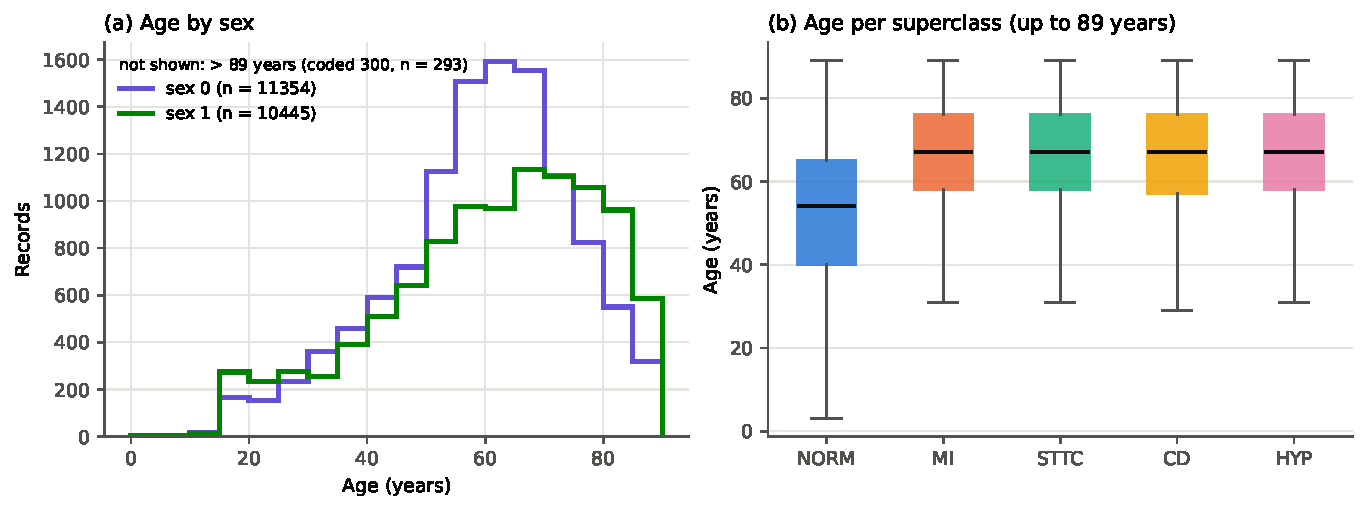
\includegraphics[width=\textwidth,height=0.42\textheight,keepaspectratio]{figures/eda_age_sex.pdf}
\caption[Age and sex]{Demographics. (a) Age histogram by sex (sex 0 = male, sex 1 = female \cite{wagner2020ptbxl}); ages above 89 are coded 300 in the dataset and not drawn. (b) Age per superclass (box: quartiles, line: median, whiskers: 1.5 interquartile ranges).}
\label{fig:eda_age_sex}
\end{figure}
